% =========================================================================== %

\begin{frame}[t,plain]
\titlepage
\end{frame}

% =========================================================================== %

\begin{frame}{Recap: Basic Plots}
%
\begin{columns}[T]
\column{.5\linewidth}
\begin{itemize}
\item \texttt{plt.plot}
	\begin{itemize}
	\item Takes two iterables, creates xy-plot \emph{in memory}
	\item Optional arguments for colour, markers, linetype, label
	\end{itemize}
\item \texttt{plt.show}
\item \texttt{plt.title}, \texttt{plt.xlabel}, \texttt{plt.ylabel}, \texttt{plt.legend}, \texttt{plt.grid}
\item \texttt{plt.xscale}, \texttt{plt.yscale}, \texttt{plt.xlim}, \texttt{plt.ylim}
\end{itemize}
%
\column{.5\linewidth}
\begin{itemize}
\item Bar Plots (\texttt{plt.bar} and \texttt{plt.barh})
\item Pie Plots (\texttt{plt.pie})
\item Stackplots (\texttt{plt.stackplot})
\item Scatterplots (\texttt{plt.scatter})
\item Quiver Plots (\texttt{plt.quiver})
\item ... and some more
\end{itemize}
\end{columns}
%
\begin{center}
	\emph{Any Questions?}
\end{center}
%
\end{frame}

% =========================================================================== %

\begin{frame}[fragile]{Chapter 10}
%
\begin{itemize}
\item Multiplots
\item Object Oriented Approach
\item 3D Plots
\item Saving Plots into Files
\end{itemize}
%
\end{frame}

% =========================================================================== %

\begin{frame}[fragile]{Multiplots}
%
\begin{itemize}
\item Multiple plots in one window
\item Command \texttt{plt.subplot}
	\begin{itemize}
	\item Defines a grid and selects the \enquote{active plot}
	\item Three Parameters: rows, columns, ID
	\item Subsequent commands affect that grid node
	\end{itemize}
\item Shortcut
	\begin{itemize}
	\item One parameter: \inPy{int rci}
	\item Each digit represents one of rows, columns, ID
	\end{itemize}
\item Optional Parameters
	\begin{itemize}
	\item \texttt{polar} (\inPy{bool}) -- draw polar plots
	\item \texttt{sharex} and \texttt{sharey} (\texttt{Axes} object -- see later) -- use same coordinate settings as other plot
	\end{itemize}
\end{itemize}
%
\end{frame}

% =========================================================================== %

\begin{frame}[fragile]
%
\begin{center}
%
\begin{codebox}[\raggedright Example: Lissajous I, width=.6\linewidth, nobeforeafter, equal height group = grpXmpLissajous]
\begin{minted}[linenos, fontsize=\scriptsize]{python3}
import math
import matplotlib.pyplot as plt

X = [x / 100 for x in range(628)]
Y = [math.sin(3 * x) for x in X]

plt.figure( figsize=(4,8) )
plt.suptitle("Lissajous-Figures")

plt.subplot(211)
plt.title("Cartesian")
plt.plot(X, Y)

plt.subplot(212, polar=True)
plt.title("Polar")
plt.plot(X, Y)

plt.show()
\end{minted}
\end{codebox}
%
\begin{tcolorbox}[title={\raggedright Output: Lissajous I}, width=.30\linewidth, nobeforeafter, equal height group = grpXmpLissajous]
	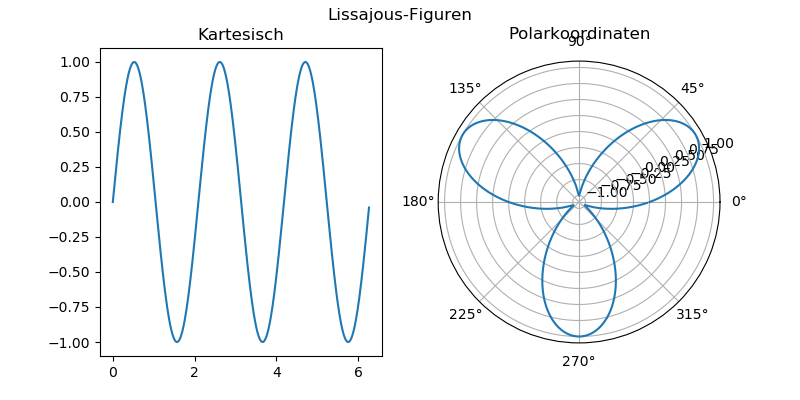
\includegraphics[width=\linewidth]{./gfx/plt-Lissajous}
\end{tcolorbox}
%
\end{center}
%
\end{frame}

% =========================================================================== %

\begin{frame}[fragile]{The Object-Oriented Approach to MatPlotLib/PyPlot}
%
\begin{itemize}
\item Idea: plots and the elements thereof are objects
\item Allows more comfortable/intuitive composition of plots
\item Dynamic evolution of plots (\eg on trigger, zoom in)
\item Primary objects: \texttt{Figure} and \texttt{AxesSubplot}
	\begin{itemize}
	\item \texttt{Figure}: window containing the plots
	\item \texttt{AxesSubplot}: rectangular region in the window where a plot can be placed
	\item Get these objects via \texttt{fig = plt.figure()} and \texttt{ax = fig.add\_subplot()}
	\end{itemize}
\item All objects provide methods for changing them
	\begin{itemize}
	\item E.\;g. \texttt{AxesSubplot}: \texttt{plot}, \texttt{bar}, \texttt{pie}, ...
	\item E.\;g. \texttt{Figure}: \texttt{suptitle}, \texttt{add\_subplot}, \texttt{show}
	\end{itemize}
\item \texttt{show} behaves differently
	\begin{itemize}
	\item \texttt{plt.show()} shows all figures at once, waits till all are closed
	\item \texttt{fig.show()} shows only the figure \texttt{fig}
	\end{itemize}
\end{itemize}
%
\end{frame}

% =========================================================================== %

\begin{frame}[fragile]
%
\begin{codebox}[Example: Lissajous II]
\begin{minted}[linenos, fontsize=\scriptsize]{python3}
import math
import matplotlib.pyplot as plt

X = [x / 100 for x in range(628)]; Y = [math.sin(3 * x) for x in X]

fig = plt.figure(figsize=(4,8))
fig.suptitle("Lissajous-Figures")

crt = fig.add_subplot(1, 2, 1)
crt.set_title("Cartesian")
crt.plot(X, Y)

pol = fig.add_subplot(1, 2, 2, projection="polar")
pol.set_title("Polar")
pol.plot(X, Y)

fig.show()
print("This will be printed while the plots are already portrayed (show does not wait)")
input()
\end{minted}
\end{codebox}
%
\end{frame}

% =========================================================================== %

\begin{frame}[fragile]{Gridspecs}
%
\begin{itemize}
\item Refined control where to place subplots
\item Grid structure where you can \enquote{select} multiple cells
\item Get via \texttt{gs = fig.add\_gridspec(rows, columns)}
\item Use when creating a new subplot: \inPy{ax = fig.add_subplot(gs[...])}
	\begin{itemize}
	\item Index can be a \inPy{tuple} of \inPy{int}s: \texttt{gs[row, column]} ...
	\item ... or a \inPy{tuple} of \inPy{slice}s:\inPy{gs[row_start : row_end, column]}
	\end{itemize}
\end{itemize}
%
\end{frame}

% =========================================================================== %

\begin{frame}[fragile]{The Object-Oriented Approach to MatPlotLib/PyPlot}
%
\begin{itemize}
\item Idea: plots and the elements thereof are objects
\item Allows more comfortable/intuitive composition of plots
\item Dynamic evolution of plots (\eg on trigger, zoom in)
\item Primary objects: \texttt{Figure} and \texttt{AxesSubplot}
	\begin{itemize}
	\item \texttt{Figure}: window containing the plots
	\item \texttt{AxesSubplot}: rectangular region in the window where a plot can be placed
	\item Get these objects via \texttt{fig = plt.figure()} and \texttt{ax = fig.add\_subplot()}
	\end{itemize}
\item All objects provide methods for changing them
	\begin{itemize}
	\item E.\;g. \texttt{AxesSubplot}: \texttt{plot}, \texttt{bar}, \texttt{pie}, ...
	\item E.\;g. \texttt{Figure}: \texttt{suptitle}, \texttt{add\_subplot}, \texttt{show}
	\end{itemize}
\item \texttt{show} behaves differently
	\begin{itemize}
	\item \texttt{plt.show()} shows all figures at once, waits till all are closed
	\item \texttt{fig.show()} shows only the figure \texttt{fig}
	\end{itemize}
\end{itemize}
%
\end{frame}

% =========================================================================== %

\begin{frame}
%
\begin{tcolorbox}[title=2D Normal Distribution]
\begin{center}
	\begin{minipage}{.45\linewidth}
	\includegraphics[width=\linewidth]{./gfx/plt-gauss2d}	
	\end{minipage}
	\begin{minipage}{.5\linewidth}
	\begin{itemize}
	\item 3$\times$3 grid
	\item scatterplot: 2$\times$2 tile in the grid, beginning at coordinate (0, 0)
	\item x-histogram: 2$\times$1 tile in the grid, beginning at coordinate (2, 0)
	\item y-histogram: 1$\times$2 tile in the grid, beginning at coordinate (0, 2)
	\item empty tile at coordinate (2, 2)
	\end{itemize}
	\end{minipage}
\end{center}
\end{tcolorbox}
%
\end{frame}

% =========================================================================== %

\begin{frame}[fragile]
%
\begin{codebox}[Code: 2D Normal Distribution ...]
\begin{minted}[linenos, fontsize=\scriptsize]{python3}
import random
import matplotlib.pyplot as plt

N      = 1000
X      =   50; sigmaX =    5
Y      =   40; sigmaY =   10
dataX = [random.gauss(X, sigmaX) for _ in range(N)]
dataY = [random.gauss(Y, sigmaY) for _ in range(N)]

fig = plt.figure(figsize=(8, 8))
gs  = fig.add_gridspec(3, 3)

fig.suptitle("2D Normal Distribution")
fig.subplots_adjust(wspace=0.2, hspace=0.3)  # set spacing between subplots

axScatter = fig.add_subplot(gs[0:2, 0:2])
axScatter.set_xlim(0, 100)
axScatter.set_ylim(0, 100)
axScatter.set_xlabel("x")
\end{minted}
\end{codebox}
%
\end{frame}

% =========================================================================== %

\begin{frame}[fragile]
%
\begin{codebox}[... continued]
\begin{minted}[linenos, firstnumber=last, fontsize=\scriptsize]{python3}
axHistX   = fig.add_subplot(gs[ 2 , 0:2], sharex=axScatter)
axHistY   = fig.add_subplot(gs[0:2,  2 ], sharey=axScatter)

axScatter.scatter(dataX, dataY, marker=".")
axHistX.hist(dataX, orientation='vertical'  , bins=20)
axHistY.hist(dataY, orientation='horizontal', bins=20)

fig.show()
\end{minted}
\end{codebox}
%
\end{frame}

% =========================================================================== %

\begin{frame}[fragile]{Naming Convention}
%
\begin{itemize}
\item Simple approach: \texttt{plt.property} (\eg \texttt{plt.title})
\item Object oriented approach: \texttt{obj.set\_property} (and \texttt{obj.get\_property})
\item In particular
	\begin{itemize}
	\item \texttt{set\_title}
	\item \texttt{set\_xlabel}, \texttt{set\_ylabel}
	\item \texttt{set\_xscale}, \texttt{set\_yscale}
	\item \texttt{set\_xlim}, \texttt{set\_ylim}
	\item ... and the respective getters
	\end{itemize}
\item This also holds for Object Oriented Programming in general, across languages
\end{itemize}
%
\end{frame}

% =========================================================================== %

\begin{frame}[fragile]{Tickmarks}
%
\begin{itemize}
\item \enquote{Lines on the axis}
\item Major and minor ticks
\item Methods \texttt{ax.set\_xticks(positions, minor)} and \texttt{ax.set\_yticks}
	\begin{itemize}
	\item \texttt{positions}: iterable (container) with values where to place a tick
	\item \texttt{minor}: \inPy{bool}, marks the \texttt{positions} as minor ticks. Default: \inPy{false}
	\end{itemize}
\item Methods \texttt{ax.set\_xticklabels(texts, minor)}
	\begin{itemize}
	\item \texttt{texts}: iterable of \inPy{str}ings to place at the tickmarks
	\item \texttt{minor}: as above
	\item Optional parameter \texttt{fontdict}: \inPy{dict} with additional format parameters
		\begin{itemize}
		\item \inPy{'fontsize'} \thus \inPy{int}
		\item \inPy{'fontweight'} \thus \inPy{str}, \eg \inPy{'bold'} or \inPy{'bold'}
		\item ...
		\item \url{https://matplotlib.org/3.3.1/api/text_api.html#matplotlib.text.Text}
		\end{itemize}
	\end{itemize}
\end{itemize}
%
\end{frame}

% =========================================================================== %

\begin{frame}[fragile]{FuncFormatter}
%
\begin{itemize}
\item Automatically generate tick labels according to a function
	\begin{itemize}
	\item Input: \inPy{(value, number_of_tick)}
	\item Output: \inPy{str}ing
	\end{itemize}
\item Needs to be wrapped in MatPlotLib interface
\item Dedicated object \texttt{FuncFormatter}
	\begin{itemize}
	\item import from matplotlib.ticker
	\item Use as a function
	\end{itemize}
\end{itemize}
%
\end{frame}

% =========================================================================== %

\begin{frame}[fragile]
%
\begin{codebox}[Example: Tickmarks, width=.65\linewidth, nobeforeafter, equal height group = grpXmpFormatter]
\begin{minted}[linenos, fontsize=\scriptsize]{python3}
from matplotlib.ticker import FuncFormatter
import matplotlib.pyplot as plt

x = list(range(4))
money = [1.5e5, 2.5e6, 5.5e6, 2.0e7]

fig = plt.figure(figsize=(4,7))
ax = fig.subplots()
ax.bar(x, money)

ax.set_xticks(x)
ax.set_xticklabels(['Bill', 'Fred', 'Mary', 'Sue'],
    fontdict={'fontsize' :15, 'fontweight' : 'bold'})

myTicks   = lambda x, pos : f"{x*1e-6:1.1f}M, #{pos}"
formatter = FuncFormatter(myTicks)
ax.yaxis.set_major_formatter(formatter)

plt.show()
\end{minted}
\end{codebox}
%
\begin{tcolorbox}[title=Output: Tickmarks, width=.32\linewidth, nobeforeafter, equal height group = grpXmpFormatter]
	\hspace{-13pt}
	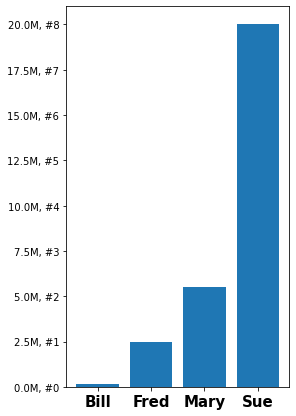
\includegraphics[width=1.22\linewidth]{./gfx/plt-TicksFormatter}
\end{tcolorbox}
%
\end{frame}

% =========================================================================== %

